\chapter{Concepção de pesquisa através do \textit{Educational Design Research}} \label{ch:edr}

O \textit{Educational Design Research} (EDR) é uma abordagem metodológica que visa integrar a teoria e a prática para desenvolver soluções eficazes e inovadoras em contextos educacionais. A essência do EDR reside no reconhecimento de que os desafios enfrentados por organizações e comunidades educacionais são complexos e multifacetados, indo além de meros problemas teóricos e demandando soluções práticas que atendam às necessidades reais.

Essa abordagem enfatiza uma perspectiva holística, ou seja, a compreensão dos problemas educacionais deve considerar os diferentes aspectos e contextos envolvidos. A colaboração entre pesquisadores e partes interessadas é valorizada, uma vez que essas últimas trazem consigo experiências práticas, percepções e conhecimentos do mundo real, complementando as visões teóricas dos pesquisadores. A sinergia resultante entre teoria e prática é fundamental para o desenvolvimento de soluções que possam ser efetivamente implementadas e que produzam impactos significativos no ambiente educacional.

Na Seção \ref{ch:edrtrue} faremos um apanhado geral sobre o EDR que foi o método de pesquisa abordado nesta dissertação. Por fim, na Seção \ref{ch:edrmpeac} faremos uma breve descrição das concepções do EDR do ponto de vista do nosso gurpo de pesquisa: Métodos e Processos de Ensino e Aprendizagem de Ciências (MPEAC).

\section{\textit{Educational Design Research}} \label{ch:edrtrue}

De acordo com \citeonline[p.326]{McKenney2018}, o EDR é caracterizado por seu compromisso em conjuntamente desenvolver percepções teóricas e soluções práticas em contextos reais, em colaboração com as partes interessadas. Este método se distingue das demais abordagens de pesquisa científica ao buscar uma abordagem integrada e aplicada, onde a teoria e a prática são desenvolvidas de forma simultânea e complementar, resultando em soluções eficazes e relevantes para as questões reais enfrentadas pela comunidade de interesse.

O uso do EDR proporciona uma análise detalhada e abrangente de diversas formas de soluções no contexto educacional, englobando processos, programas, políticas e produtos educacionais. Conforme ressaltado por \citeonline{McKenney2018}, o EDR oferece uma abordagem flexível e adaptável, permitindo que os pesquisadores se concentrem em diferentes aspectos do cenário educacional, de acordo com suas necessidades e objetivos específicos de pesquisa.

Ao adotar o EDR como metodologia de pesquisa, os investigadores tem a oportunidade de explorar e descrever a concepção, desenvolvimento, implementação e avaliação de soluções educacionais com uma perspectiva mais integrada, conforme destacado por \citeonline{plomp2013educational}. Essa abordagem possibilita uma visão mais completa e aprofundada dos desafios enfrentados e das possíveis maneiras de superá-los.

Um aspecto relevante do EDR é a sua aplicação em projetos de intervenção, nos quais programas e práticas educacionais são desenvolvidos e testados em contextos reais. Esse enfoque permite uma investigação profunda das soluções propostas, incluindo sua viabilidade, eficácia e impacto nos resultados de aprendizagem dos alunos, bem como na dinâmica da sala de aula e na experiência do professor.

Outro campo de estudo abarcado pelo EDR é a análise de políticas educacionais, identificando seus pontos fortes, desafios e impactos em nível macro nas instituições de ensino e na sociedade em geral. Isso inclui a investigação das políticas de inclusão, avaliação educacional, formação de professores, entre outras, contribuindo para a compreensão dos resultados e aprimoramento das melhores práticas.

Além disso, a abordagem do EDR também pode ser aplicada na análise de produtos educacionais, como softwares, aplicativos, recursos didáticos e materiais instrucionais. Ao adotar essa perspectiva, os pesquisadores podem avaliar a usabilidade, eficácia e adequação desses produtos para apoiar o processo de ensino e aprendizagem, conforme mencionado por \citeonline{anderson2012design}.

É importante enfatizar que o EDR abrange várias variações e abordagens específicas, de acordo com as áreas de estudo e as demandas de pesquisa. No entanto, em um contexto geral, o EDR oferece uma perspectiva integradora e colaborativa, na qual pesquisadores, educadores e demais partes interessadas trabalham juntos para desenvolver soluções mais eficazes e adaptadas ao contexto educacional. Ao fazer isso, o EDR contribui para o avanço da pesquisa educacional e para a melhoria contínua da qualidade da educação.

Dizemos que o EDR é definido como um tipo de pesquisa que emprega o desenvolvimento iterativo de soluções para abordar problemas educacionais práticos e complexos, permitindo uma investigação empírica que resulta em uma compreensão teórica que pode informar o trabalho de outros pesquisadores \cite[p.326]{McKenney2018}. Os objetivos e métodos do EDR estão estreitamente alinhados com o mundo real e suas várias facetas.

O EDR se preocupa em desenvolver o que \citeonline{Legemann2002} denominou de conhecimento utilizável, tornando os resultados da pesquisa relevantes para a prática educacional. Esse conhecimento útil é produzido ao longo da pesquisa e é fundamentalmente importante compartilhá-lo com outros pesquisadores e profissionais, destacando a importância da troca de informações para o progresso e desenvolvimento teórico na área.

Essa abordagem de pesquisa, com base no desenvolvimento iterativo de soluções e uma investigação empírica, contribui para a produção de conhecimentos aplicáveis e pertinentes ao contexto educacional, favorecendo uma interação contínua entre a teoria e a prática.

De acordo com \citeonline[p.5]{DBRC2003}, uma boa pesquisa baseada em \textit{design} deve apresentar cinco importantes características. A primeira é a interligação entre os objetivos principais do \textit{design} de ambientes de aprendizagem e o desenvolvimento de teorias ou protótipos de aprendizagem. Segundo \citeonline{DBRC2003}, essa integração permite que as soluções educacionais propostas sejam fundamentadas em bases teóricas sólidas.

A segunda característica ressaltada por \citeonline{DBRC2003} é que o desenvolvimento e a pesquisa devem ocorrer em etapas cíclicas e contínuas de projeto, execução, análise e redesenho. Esse processo iterativo permite ajustes e melhorias contínuas nas intervenções educacionais, de acordo com os resultados obtidos.

Em terceiro lugar, \citeonline{DBRC2003} enfatizam que a pesquisa baseada em \textit{design} deve levar a teorias compartilháveis que possam auxiliar outros pesquisadores da área. Essa colaboração e disseminação do conhecimento contribuem para o avanço da comunidade acadêmica e para o crescimento do campo educacional, conforme mencionado por \citeonline{Collins1992} e \citeonline{Coob2001}.

A quarta característica destacada por \citeonline{DBRC2003} ressalta a importância de documentar detalhadamente como o \textit{design} funciona em ambientes reais de aprendizagem. Isso inclui não apenas relatar o sucesso ou fracasso da intervenção, mas também descrever as interações e processos envolvidos na compreensão das questões de aprendizagem.

Por fim, a quinta característica ressaltada por \citeonline{DBRC2003} é que o desenvolvimento da pesquisa deve se basear em métodos que possam documentar desde a concepção e implementação do \textit{design} até a análise dos resultados alcançados. Essa abordagem metodológica rigorosa garante a robustez e a confiabilidade da pesquisa baseada em \textit{design}. 

Ainda, segundo o \citeonline[p.5]{DBRC2003}: 

\begin{quoting} 
[leftmargin=4cm, rightmargin=0cm]
\noindent
É importante ressaltar que a pesquisa baseada em design vai além do mero projeto e teste de intervenções específicas. As intervenções incorporam afirmações teóricas específicas sobre o ensino e aprendizagem, e refletem um compromisso com a compreensão das relações entre teoria, projeto de produtos, e prática. Ao mesmo tempo, pesquisas sobre intervenções específicas podem contribuir para teorias de aprendizagem e ensino.
\end{quoting}

Os resultados obtidos através do EDR são cuidadosamente analisados e discutidos, permitindo que ocorra uma reaplicação das soluções, incorporando as modificações e aprimoramentos necessários. Esse processo iterativo é fundamental para a melhoria contínua das intervenções e para o aperfeiçoamento das soluções propostas ao longo do tempo.

É essencial que todo o processo de pesquisa seja documentado de forma rigorosa e clara. A documentação permite que outros pesquisadores compreendam detalhadamente o estudo realizado, possam replicá-lo e adaptá-lo para suas próprias realidades e contextos educacionais.

O compartilhamento dos resultados e das experiências é um aspecto crucial do EDR. Ao disponibilizar as descobertas, lições aprendidas e as soluções desenvolvidas, a comunidade acadêmica e os profissionais da educação podem se beneficiar das contribuições uns dos outros, enriquecendo o conhecimento coletivo e promovendo avanços no campo educacional.

Portanto, o EDR é um processo cíclico e colaborativo, onde a pesquisa, o \textit{design}, a implementação, a análise e a documentação são partes essenciais. Através desse enfoque, o EDR visa gerar e compartilhar conhecimento aplicado que contribua para o aprimoramento contínuo da educação e para o benefício da sociedade como um todo. A Figura \ref{fig:mattaeboa} representa, de forma esquemática, o processo cíclico do EDR.

\begin{figure}[H]
\caption{Processo cíclico do EDR.}
  \label{fig:mattaeboa}
  \centering
  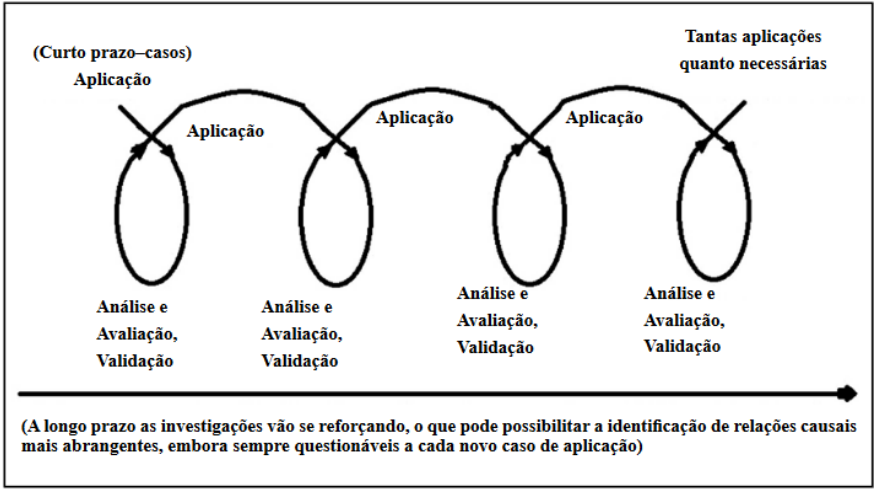
\includegraphics[width=0.8\textwidth]{fig/mattaeboa.png}
  \caption*{Fonte: Retirado de \citeonline[p.29]{MATTA2014}.}
\end{figure}

Resumidamente, segundo \cite{alves2018}, \cite{MATTA2014} e \cite{McKenney2018}, o EDR destaca-se das demais modalidades de investigação nas áreas de Educação ou Ensino devido a um conjunto específico de características distintivas. Estas incluem sua abordagem teoricamente orientada, seu caráter intervencionista, a ênfase na colaboração, a capacidade de resposta às necessidades contextuais e o processo iterativo. 

\begin{table}[H]
\centering
\caption{Características do EDR} \label{tab:carctEDR}
\begin{tabular}{p{5.8cm} p{6.7cm}}
\hline 
\textbf{Teoricamente Orientada} & Constituída a partir dos princípios de design já existentes.\\ 
\hline 
\textbf{Intervencionista} & Inclui a implementação do produto criado.\\ 
\hline 
\textbf{Colaborativa} & Pode ser conduzida em diferentes graus de colaboração entre o pesquisador e/ou profissional que atua em um contexto educacional específico.\\ 
\hline 
\textbf{Responsiva} & Suas pesquisas são conduzidas em ambientes complexos e mutáveis ao longo do tempo.\\ 
\hline 
\textbf{Iterativa} & O ciclo de pesquisa evolui continuamente no tempo.\\ 
\hline 
\end{tabular}
\caption*{Fonte: Criação do Autor baseado no texto de \citeonline{alves2018}.}
\end{table}

Essa diversidade de elementos torna o EDR uma abordagem singular e eficaz na abordagem e solução de questões práticas enfrentadas em contextos educacionais. Na Tabela \ref{tab:carctEDR} apresentamos as características presentes no EDR, de forma resumida.

\section{EDR no MPEAC} \label{ch:edrmpeac}

Na perspectiva do grupo de pesquisa MPEAC, a ênfase reside no desenvolvimento de uma solução aplicada para um problema real e específico \cite{alves2018}. Além disso, há um comprometimento com a efetiva implementação e sustentação das soluções já concebidas.

\begin{table}[H]
\ABNTEXfontereduzida % Reduzir tamanho da fonte conforme normas ABNT
\centering % Centralizar a tabela
\caption{Etapas do EDR no MPEAC}
\label{tab:etapas-edr-mpeac}
\begin{tabularx}{\linewidth}{@{}lX@{}} % Definir a largura das colunas
\toprule
\textbf{1)} & Identificar/definir uma problemática educacional real e localizada em um contexto concreto de ensino e aprendizagem.\\
\midrule
\textbf{2)} & Especificar uma possível solução para a problemática delimitada anteriormente.\\
\midrule
\textbf{3)} & Desenvolver uma possível solução de acordo com a especificação elaborada na etapa anterior.\\
\midrule
\textbf{4)} & Implementar na prática a solução desenvolvida na etapa anterior.\\
\midrule
\textbf{5)} & Analisar a implementação da solução proposta com vistas ao seu aperfeiçoamento/viabilidade e buscar contribuições teóricas para a área de ensino.\\
\midrule
\textbf{6)} & Observar fenômenos de ensino e aprendizagem com vistas a contribuir para o conhecimento teórico da área.\\
\bottomrule
\end{tabularx}
\source{Adaptado de \citeonline[p. 48]{alves2018}.} % Fonte da tabela
\end{table}

A Tabela \ref{tab:etapas-edr-mpeac} apresenta as etapas do EDR de acordo com a perspectiva do grupo de pesquisa, conforme descrito por \citeonline{alves2018}. Essas etapas representam um processo metodológico sistemático para a concepção, implementação e análise de intervenções educacionais, visando aprimorar o processo de ensino e aprendizagem de forma embasada e estruturada.

A primeira etapa consiste na identificação e definição de uma problemática educacional real e contextualizada. Nessa fase, os pesquisadores buscam compreender os desafios e as necessidades enfrentadas em um ambiente de ensino específico, a fim de delimitar o escopo da pesquisa e estabelecer os objetivos a serem alcançados.

Em seguida, na segunda etapa, é especificada uma possível solução para a problemática identificada. Essa etapa envolve a proposição de estratégias e abordagens que possam ser aplicadas de forma concreta para enfrentar o problema educacional em questão.

Na terceira etapa, acontece o desenvolvimento da solução proposta, transformando-a em um plano prático. Nesse estágio, os pesquisadores detalham e elaboram as intervenções educacionais com base nas especificações previamente definidas.

A implementação da solução ocorre na quarta etapa, na qual as intervenções educacionais são colocadas em prática em um ambiente real de ensino e aprendizagem. Durante essa fase, os pesquisadores podem ajustar e adaptar a intervenção de acordo com as necessidades e desafios identificados na execução.

Na quinta etapa, os pesquisadores analisam criticamente a implementação da solução, buscando identificar pontos fortes, fraquezas e oportunidades de melhoria. Essa análise detalhada visa aperfeiçoar a intervenção e, ao mesmo tempo, contribuir para o avanço do conhecimento teórico na área de ensino e aprendizagem.

Por fim, na sexta etapa, a observação de fenômenos de ensino e aprendizagem busca oferecer uma contribuição valiosa para o conhecimento teórico no campo educacional. Essa etapa visa ampliar a compreensão dos processos educacionais envolvidos na intervenção e, potencialmente, propor teorias ou modelos que possam ser aplicados em outros contextos educacionais.

As etapas do EDR no MPEAC são concebidas como um ciclo iterativo (Figura \ref{fig:mattaeboa}), no qual as aprendizagens e descobertas obtidas em cada fase contribuem para aprimorar as etapas subsequentes. Esse processo dinâmico de investigação permite uma abordagem holística para a resolução de problemas educacionais complexos, promovendo a conexão entre teoria e prática para o avanço da educação.
